% !TeX program = xelatex
\documentclass[10pt]{beamer}

\usetheme{metropolis}

%\usepackage{pgfplots}
%\usepgfplotslibrary{dateplot}
\usepackage{pgfopts}
\usepackage{amsmath}
\usepackage{structuralanalysis}
\usepackage{tikz}
\usepackage{tikz-3dplot}
\usepackage{mathtools}

\makeatletter
\def\user@resume{resume}
\def\user@intermezzo{intermezzo}
%
\newcounter{previousequation}
\newcounter{lastsubequation}
\newcounter{savedparentequation}
\setcounter{savedparentequation}{1}
% 
\renewenvironment{subequations}[1][]{%
	\def\user@decides{#1}%
	\setcounter{previousequation}{\value{equation}}%
	\ifx\user@decides\user@resume 
	\setcounter{equation}{\value{savedparentequation}}%
	\else  
	\ifx\user@decides\user@intermezzo
	\refstepcounter{equation}%
	\else
	\setcounter{lastsubequation}{0}%
	\refstepcounter{equation}%
	\fi\fi
	\protected@edef\theHparentequation{%
		\@ifundefined {theHequation}\theequation \theHequation}%
	\protected@edef\theparentequation{\theequation}%
	\setcounter{parentequation}{\value{equation}}%
	\ifx\user@decides\user@resume 
	\setcounter{equation}{\value{lastsubequation}}%
	\else
	\setcounter{equation}{0}%
	\fi
	\def\theequation  {\theparentequation  \alph{equation}}%
	\def\theHequation {\theHparentequation \alph{equation}}%
	\ignorespaces
}{%
%  \arabic{equation};\arabic{savedparentequation};\arabic{lastsubequation}
\ifx\user@decides\user@resume
\setcounter{lastsubequation}{\value{equation}}%
\setcounter{equation}{\value{previousequation}}%
\else
\ifx\user@decides\user@intermezzo
\setcounter{equation}{\value{parentequation}}%
\else
\setcounter{lastsubequation}{\value{equation}}%
\setcounter{savedparentequation}{\value{parentequation}}%
\setcounter{equation}{\value{parentequation}}%
\fi\fi
%  \arabic{equation};\arabic{savedparentequation};\arabic{lastsubequation}
\ignorespacesafterend
}
\makeatother

\title{AE 737 - Mechanics of Damage Tolerance}
\subtitle{Lecture 2}
\date{21 January 2016}
\author{Dr. Nicholas Smith}
\institute{Wichita State University, Department of Aerospace Engineering}
% \titlegraphic{\hfill\includegraphics[height=1.5cm]{logo/logo}}

\begin{document}

\maketitle

\begin{frame}
  \frametitle{outline}
  \setbeamertemplate{section in toc}[sections numbered]
  \tableofcontents[hideallsubsections]
\end{frame}

\begin{frame}{office hours}
  \begin{itemize}
  \item I will e-mail everyone in the course a Doodle link we can use to find the optimal office hours
  \item Let me know if you do not receive the e-mail, you may need to update your information in Blackboard
  \item Take advantage of office hours, this is time that I have already set aside for you
  \item If the regular office hours do not work for your schedule, send me an e-mail and we can work out a time to meet
  \item While in person visits are often the most helpful, I will always try to answer questions as best as I can via e-mail
  \end{itemize}
\end{frame}

\section{Fracture Mechanics}

\begin{frame}{fracture mechanics}
	\begin{itemize}
		\item \emph{Linear Elastic Fracture Mechanics} is the study of the propagation of cracks in materials
		\item There are some corrections we add to account for plasticity
		\item In this course we will not follow the full mathematical development of fracture mechanics (there is a separate course dedicated to that)
		\item Instead we will take some results and apply them
	\end{itemize}
\end{frame}

\begin{frame}{fracture mechanics}
	\begin{itemize}
		\item In fracture mechanics we consider three different modes
		\item Mode I is known as the "opening mode"
		\item Mode II is known as the "sliding mode"
		\item Mode III is known as the "tearing mode"
	\end{itemize}
\end{frame}

\begin{frame}{fracture mechanics}
	\begin{figure}
	\def\svgwidth{\linewidth}
	\input{Fracture_modes_v2.pdf_tex}
	\end{figure}
\end{frame}

\section{Stress Intensity}

\begin{frame}{stress intensity}
	\begin{itemize}
		\item A key finding from Linear Elastic Fracture Mechanics (LEFM) is known as the \emph{Stress Intensity Factor}
		\item The stress intensity factor is often written in this form
		\begin{equation*}
		K = \sigma\sqrt{\pi a} \beta
		\end{equation*}
		\item Where $K$ is the stress intensity factor, $\sigma$ is the applied stress, $a$ is the crack length, and $\beta$ is a dimensionless parameter depending on geometry
		\item Be careful that although the notation is similar, the \emph{Stress Intensity Factor} is different from the \emph{Stress Concentration Factor} from strength of materials
		\item We are usually most concerned with Mode I, but there will be a unique stress intensity factor for each mode, we label these $K_I$, $K_{II}$, and $K_{III}$
		\item If no subscript is given, assume Mode I
	\end{itemize}
\end{frame}

\begin{frame}{stress intensity}
	\begin{itemize}
		\item For brittle materials (where "linear" fracture mechanics assumptions hold true) we can find the full stress field near the crack in terms of the stress intensity factor
		\begin{align*}
		\sigma_x &= \frac{K_I}{\sqrt{2\pi r}} \cos \frac{\theta}{2} \left(1-\sin \frac{\theta}{2}\sin \frac{3\theta}{2}\right)\\
		\sigma_y &= \frac{K_I}{\sqrt{2\pi r}} \cos \frac{\theta}{2} \left(1+\sin \frac{\theta}{2}\sin \frac{3\theta}{2}\right)\\
		\tau_{xy} &= \frac{K_I}{\sqrt{2\pi r}} \sin \frac{\theta}{2} \cos \frac{\theta}{2}\cos \frac{3\theta}{2}
		\end{align*}
	\end{itemize}
\end{frame}

\begin{frame}{stress intensity}
	\begin{itemize}
		\item Similarly for Mode II we find
		\begin{align*}
		\sigma_x &= \frac{-K_{II}}{\sqrt{2\pi r}} \sin \frac{\theta}{2} \left(2+\cos \frac{\theta}{2}\cos \frac{3\theta}{2}\right)\\
		\sigma_y &= \frac{K_{II}}{\sqrt{2\pi r}} \sin \frac{\theta}{2} \cos \frac{\theta}{2}\cos \frac{3\theta}{2}\\
		\tau_{xy} &= \frac{K_{II}}{\sqrt{2\pi r}} \cos \frac{\theta}{2} \left(1-\sin \frac{\theta}{2}\sin \frac{3\theta}{2}\right)
		\end{align*}
	\end{itemize}
\end{frame}

\begin{frame}{stress intensity}
	\begin{itemize}
		\item And for Mode III
		\begin{align*}
		\tau_{xz} &= \frac{-K_{III}}{\sqrt{2\pi r}} \sin \frac{\theta}{2} \\
		\tau_{yz} &= \frac{K_{III}}{\sqrt{2\pi r}} \cos \frac{\theta}{2} 
		\end{align*}
	\end{itemize}
\end{frame}

\section{Common stress intensity factors}

\begin{frame}{center crack, infinite width}
	\begin{figure}[H]
		\begin{equation}
		K_I = \sigma \sqrt{\pi a}
		\end{equation}
		\centering
		\begin{tikzpicture}
		\begin{scope}[scale=1.5]
		\point{a}{0}{2};
		\point{b}{6}{2};
		\point{c}{0}{-3};
		\point{d}{6}{-3};
		\draw (0,0) -- (0,1) -- (4,1) -- (4,-1) -- (0,-1) -- (0,0);
		\draw (1.5,0) -- (2.5,0);
		\draw node at (2,0.2) {2a};
		\lineload{3}{a}{b}[-.5][-.5];
		\draw node at (2,2) {$\sigma$};
		\lineload{3}{c}{d}[.5][.5];
		\draw node at (2,-2) {$\sigma$};
		\end{scope}
		\end{tikzpicture}
	\end{figure}
\end{frame}

\begin{frame}{center crack, finite width}
	\begin{figure}[H]
		\begin{equation}
		K_I = \sigma \sqrt{\pi a} \sqrt{\sec (\pi a/W)}
		\end{equation}
		\centering
		\begin{tikzpicture}
		\begin{scope}[scale=1.5]
		\point{a}{0}{2};
		\point{b}{6}{2};
		\point{c}{0}{-3};
		\point{d}{6}{-3};
		\draw (0,0) -- (0,1) -- (4,1) -- (4,-1) -- (0,-1) -- (0,0);
		\draw (1.5,0) -- (2.5,0);
		\draw node at (2,0.2) {2a};
		\lineload{3}{a}{b}[-.5][-.5];
		\draw node at (2,2) {$\sigma$};
		\lineload{3}{c}{d}[.5][.5];
		\draw node at (2,-2) {$\sigma$};
		\draw[->] (1.5,-0.5) -- (0,-0.5);
		\draw[->] (2.5,-0.5) -- (4,-0.5);
		\draw node at (2,-0.5) {$W$};
		\end{scope}
		\end{tikzpicture}
	\end{figure}
\end{frame}

\begin{frame}{edge crack, semi-infinite width}
	\begin{figure}[H]
		\begin{equation}
		K_I = 1.12 \sigma \sqrt{\pi a}
		\end{equation}
		\centering
		\begin{tikzpicture}
		\begin{scope}[scale=1.5]
		\point{a}{0}{2};
		\point{b}{6}{2};
		\point{c}{0}{-3};
		\point{d}{6}{-3};
		\draw (0,0) -- (0,1) -- (4,1) -- (4,-1) -- (0,-1) -- (0,0);
		\draw (0,0) -- (0.5,0);
		\draw node at (0.25,0.2) {a};
		\lineload{3}{a}{b}[-.5][-.5];
		\draw node at (2,2) {$\sigma$};
		\lineload{3}{c}{d}[.5][.5];
		\draw node at (2,-2) {$\sigma$};
%		\draw[->] (1.5,-0.5) -- (0,-0.5);
%		\draw[->] (2.5,-0.5) -- (4,-0.5);
%		\draw node at (2,-0.5) {$W$};
		\end{scope}
		\end{tikzpicture}
	\end{figure}
\end{frame}

\begin{frame}{edge crack, finite width}

	\begin{figure}[H]
		\begin{equation}
		K_I = \sigma \sqrt{\pi a}\left[1.12 - 0.231 \frac{a}{W} + 10.55 \left(\frac{a}{W}\right)^2 - 21.72 \left(\frac{a}{W}\right)^3 + 30.39 \left(\frac{a}{W}\right)^4\right]
		\end{equation}
		\centering
		\begin{tikzpicture}
		\begin{scope}[scale=1.5]
		\point{a}{0}{2};
		\point{b}{6}{2};
		\point{c}{0}{-3};
		\point{d}{6}{-3};
		\draw (0,0) -- (0,1) -- (4,1) -- (4,-1) -- (0,-1) -- (0,0);
		\draw (0,0) -- (0.5,0);
		\draw node at (0.25,0.2) {a};
		\lineload{3}{a}{b}[-.5][-.5];
		\draw node at (2,2) {$\sigma$};
		\lineload{3}{c}{d}[.5][.5];
		\draw node at (2,-2) {$\sigma$};
		\draw[->] (1.5,-0.5) -- (0,-0.5);
		\draw[->] (2.5,-0.5) -- (4,-0.5);
		\draw node at (2,-0.5) {$W$};
		\end{scope}
		\end{tikzpicture}
	\end{figure}
		
\end{frame}

\begin{frame}{offset crack}
	\begin{figure}[H]
		\centering
		\begin{tikzpicture}
		\begin{scope}[scale=1.5]
		\point{a}{0}{2};
		\point{b}{3}{2};
		\point{c}{0}{-3};
		\point{d}{3}{-3};
		\draw (0,0) -- (0,1) -- (2,1) -- (2,-1) -- (0,-1) -- (0,0);
		\draw (0.2,0) -- (0.8,0);
		\draw node at (0.15,0.1) {\small A} node at (.85,.1) {\small B} node at (.25,.5) {\small $b$};
		\draw node at (0.5,-0.2) {2a};
		\lineload{3}{a}{b}[-.5][-.5];
		\draw node at (1,2) {$\sigma$};
		\lineload{3}{c}{d}[.5][.5];
		\draw node at (1,-2) {$\sigma$};
		\draw[->] (0.7,-0.7) -- (0,-0.7);
		\draw[->] (1.3,-0.7) -- (2,-0.7);
		\draw node at (1,-0.7) {$W$};
		\draw[dashed] (.5,0) -- (.5,.8);
		\draw[->] (0.15,.5) -- (0,.5);
		\draw[->] (.35,.5) -- (.5,.5);
		\end{scope}
		\end{tikzpicture}
	\end{figure}
\end{frame}

\begin{frame}{offset crack}
	\begin{equation}
	K_{IA} = \sigma \sqrt{\pi a} \beta_c \beta_A \text{ and } K_{IB} = \sigma \sqrt{\pi a} \beta_c \beta_B
	\end{equation}
	\begin{subequations}
		\begin{align}
		\beta_c &= \sqrt{\sec \frac{\pi a}{W}}\\
		&\begin{aligned}
		\mathllap{\beta_A} &= (1-0.025\lambda^2 + 0.6\lambda^4 - \gamma \lambda^{11})\\
		&\qquad \sqrt{\sec \left(\frac{\pi \lambda}{2}\right)\frac{\sin \left(2\lambda - 4\frac{a}{W}\right)}{2\lambda - 4\frac{a}{W}}}
		\end{aligned}\\
		&\begin{aligned}
		\mathllap{\beta_B} &= (1-0.025\delta^2 + 0.06\delta^4 - \zeta \lambda^{30})\\
		&\qquad \left(1+\frac{\sqrt{\sec\left(\frac{2\pi \lambda + 1.5\pi \delta}{7}\right)-1}}{1+0.21\sin \left( 8 \tan^{-1} \left(\frac{\lambda - \delta}{\lambda + \delta}\right)^{0.9}\right)}\right)
		\end{aligned}		
		\end{align}
	\end{subequations}
\end{frame}

\begin{frame}{offset crack}
	\begin{itemize}
		\item The parameters $\lambda$, $\delta$ are given as
		\begin{subequations}[resume]
			\begin{align}
			\lambda &= \frac{a}{b}\\
			\delta &= \frac{a}{W-b}
			\end{align}
		\end{subequations}
		\item And $\gamma$ and $\zeta$ can be looked up on a table
		\begin{table}
			\centering
			\caption{Parameters for offset crack}
			\begin{tabular}{ccc}
				$\frac{b}{W}$  & $\gamma$ & $\zeta$ \\
				\hline 
				 0.1 & 0.382 & 0.114 \\ 
				 0.25 & 0.136 & 0.286 \\ 
				 0.4 & 0.0 & 0.0 \\ 
				 0.5 & 0.0 & 0.0 \\ 
			\end{tabular} 
		\end{table}
	\end{itemize}
\end{frame}

\begin{frame}{non-uniform stress distribution}
	content...
\end{frame}

\begin{frame}{edge crack, bending moment}
	\begin{figure}[H]
		\begin{equation}
		K_I = \frac{6M}{(W-a)^{3/2}} f(a/W)
		\end{equation}
		\begin{tabular}{c|ccccccc}
			$a/W$& .05 & .1 & .2 & .3 & .4 & .5 & .6 + \\ 
			$f(a/W)$& .36 & .49 & .60 & .66 & .69 & .72 & .73
		\end{tabular}
		 
		\vspace{1cm}
		
		\centering
		\begin{tikzpicture}
		\begin{scope}
		\draw (0,0) -- (0,1) -- (6,1) -- (6,-1) -- (0,-1) -- (0,0);
		\draw (3,1) -- (3,0.5);
		\draw node at (3.3,.75) {a} node at (1,0) {W};
		\draw[->] (1,0.3) -- (1,1);
		\draw[->] (1,-0.3) -- (1,-1);
		\draw[->] (6.5,0.5) arc (80:-80:0.5) node at (7.2,0) {M};
		\draw[->] (-0.5,0.5) arc (100:260:0.5) node at (-1.2,0) {M};
		\end{scope}
		\end{tikzpicture}
	\end{figure}
\end{frame}

\section{3D crack shapes}

\begin{frame}{crack depth}
	\begin{itemize}
		\item The previous stress intensity factors all assume a 2D problem
		\item Through the thickness, it is assumed that the crack length is the same
		\item In many cases this is not an accurate assumption
		\item We will now consider 3D crack shapes and their effect on the stress intensity factor
	\end{itemize}
\end{frame}

\begin{frame}{elliptical flaw}
	\begin{columns}[T]
		\begin{column}{0.48\columnwidth}
	\begin{figure}
		%\centering
		%\def\svgwidth{\columnwidth}
		%\input{3d_coord.pdf_tex}
		\tdplotsetmaincoords{75}{110}
		\begin{tikzpicture}[tdplot_main_coords,scale=1.5]
		\def\couleur{alerted text.fg}
		\def\altcouleur{example text.fg}
		\draw[fill=gray!50] (1,1,1) ellipse (0.25 and 0.5);
		\draw (2,0,0) -- (2,0,2) -- (2,2,2) -- (2,2,0) -- (2,0,0);
		\draw (2,2,0) -- (0,2,0) -- (0,2,2) -- (0,0,2) -- (2,0,2);
		\draw (2,2,2) -- (0,2,2);
		\draw [dashed] (0,0,2) -- (0,0,0) -- (0,2,0);
		\draw [dashed] (0,0,0) -- (2,0,0);
		\draw (2,0,1) -- (2,2,1) -- (0,2,1);
		\draw[dashed] (0,2,1) -- (0,0,1) -- (2,0,1);
		\end{tikzpicture}
	\end{figure}
	\end{column}
	\begin{column}{0.48\columnwidth}
		\begin{figure}
			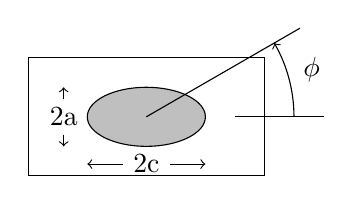
\begin{tikzpicture}
			\begin{scope}[scale=1.5]
			\draw (0,0) -- (2,0) -- (2,1) -- (0,1) -- (0,0);
			\draw[fill=gray!50] (1,0.5) ellipse (0.5 and 0.25);
			\draw node at (1,0.1) {2c};
			\draw node at (0.3,0.5) {2a};
			\draw[->] (1.2,0.1) -- (1.5,0.1);
			\draw[->] (0.8,0.1) -- (0.5,0.1);
			\draw[->] (0.3,0.65) -- (0.3,0.75);
			\draw[->] (0.3,0.35) -- (0.3,0.25);
			\draw[thin] (1.75,0.5) -- (2.5,0.5);
			\draw[thin] (1,0.5) -- (2.3,1.25);
			\draw[->] (2.25,0.5) arc (0:30:1.25);
			\draw node at (2.4,0.9) {$\phi$};
			\end{scope}
			\end{tikzpicture}
		\end{figure}
		
	\end{column}
	\end{columns}
\end{frame}

\begin{frame}{elliptical flaw}
	\begin{equation}
	K_I = \sigma \sqrt{\frac{\pi a}{Q}} \left[\sin^2 \phi + \frac{a^2}{c^2} \cos^2 \phi\right]^{1/4}
	\end{equation}
	\begin{align*}
	Q &= \Phi^2 - 0.212\left(\frac{\sigma}{\sigma_y}\right)^2 \text{(2nd term usually ignored)}\\
	\Phi &= \int_{0}^{\pi/2} \left[1-\left(\frac{c^2-a^2}{c^2}\sin^2\phi\right)\right]^2 d\phi\\
	&\approx \frac{\pi}{2} \left[1 - \frac{1}{4}\frac{c^2 - a^2}{c^2} - \frac{3}{64}\left(\frac{c^2-a^2}{c^2}\right)^2-...\right]\\
	\Phi &\approx \frac{\pi}{2} \left[1 - \frac{1}{4}\frac{c^2 - a^2}{c^2}\right] \text{(sufficient for most cases)}
	\end{align*}
\end{frame}

\begin{frame}{semi-elliptical surface flaw}
	\begin{columns}[T]
		\begin{column}{0.40\columnwidth}
			\begin{figure}
				%\centering
				%\def\svgwidth{\columnwidth}
				%\input{3d_coord.pdf_tex}
				\tdplotsetmaincoords{75}{110}
				\begin{tikzpicture}[tdplot_main_coords,scale=1.5]
				\def\couleur{alerted text.fg}
				\def\altcouleur{example text.fg}
				\draw[fill=gray!50] (1,0.5,1) arc (270:90:0.25 and 0.5);
				\draw (1,0,0) -- (1,0,2) -- (1,2,2) -- (1,2,0) -- (1,0,0);
				\draw (1,2,0) -- (-1,2,0) -- (-1,2,2) -- (-1,0,2) -- (1,0,2);
				\draw (1,2,2) -- (-1,2,2);
				\draw [dashed] (-1,0,2) -- (-1,0,0) -- (-1,2,0);
				\draw [dashed] (-1,0,0) -- (1,0,0);
				\draw (1,0,1) -- (1,2,1) -- (-1,2,1);
				\draw[dashed] (-1,2,1) -- (-1,0,1) -- (1,0,1);
				\end{tikzpicture}
			\end{figure}
		\end{column}
		\begin{column}{0.56\columnwidth}
			\begin{figure}
				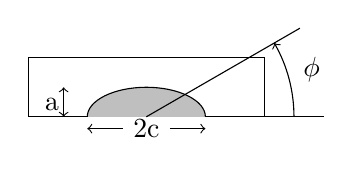
\begin{tikzpicture}
				\begin{scope}[scale=1.5]
				\draw (0,0.5) -- (2,0.5) -- (2,1) -- (0,1) -- (0,0.5);
				\draw[fill=gray!50] (.5,0.5) arc (180:0:0.5 and 0.25);
				\draw node at (1,0.4) {2c};
				\draw node at (0.2,0.6) {a};
				\draw[->] (1.2,0.4) -- (1.5,0.4);
				\draw[->] (0.8,0.4) -- (0.5,0.4);
				\draw[<->] (0.3,0.5) -- (0.3,0.75);
				\draw[thin] (1.75,0.5) -- (2.5,0.5);
				\draw[thin] (1,0.5) -- (2.3,1.25);
				\draw[->] (2.25,0.5) arc (0:30:1.25);
				\draw node at (2.4,0.9) {$\phi$};
				\end{scope}
				\end{tikzpicture}
			\end{figure}
			\begin{equation}
			K_I = \sigma \sqrt{\frac{\pi a}{Q}} \left[\sin^2 \phi + \frac{a^2}{c^2} \cos^2 \phi\right]^{1/4}(1.1)
			\end{equation}
			Note: $1.1 \approx \sqrt{1.2}$, which is known as the front surface correction factor. A more accurate correction factor is given as
			\begin{equation*}
			1 + .12\left(1-\frac{a}{c}\right)
			\end{equation*}
		\end{column}
	\end{columns}
\end{frame}

\begin{frame}{corner flaw}
	\begin{columns}[T]
		\begin{column}{0.30\columnwidth}
			\begin{figure}
				%\centering
				%\def\svgwidth{\columnwidth}
				%\input{3d_coord.pdf_tex}
				\tdplotsetmaincoords{75}{110}
				\begin{tikzpicture}[tdplot_main_coords,scale=1.5]
				\def\couleur{alerted text.fg}
				\def\altcouleur{example text.fg}
				\draw[fill=gray!50] (1,1.5,1) arc (270:180:0.25 and 0.5) -- (1,2,1) -- (1,1.5,1);
				\draw (1,1,0) -- (1,1,2) -- (1,2,2) -- (1,2,0) -- (1,1,0);
				\draw (1,2,0) -- (0,2,0) -- (0,2,2) -- (0,1,2) -- (1,1,2);
				\draw (1,2,2) -- (0,2,2);
				\draw [dashed] (0,1,2) -- (0,1,0) -- (0,2,0);
				\draw [dashed] (0,1,0) -- (1,1,0);
				\draw (1,1,1) -- (1,2,1) -- (0,2,1);
				\draw[dashed] (0,2,1) -- (0,1,1) -- (1,1,1);
				\end{tikzpicture}
			\end{figure}
		\end{column}
		\begin{column}{0.66\columnwidth}
			\begin{figure}
				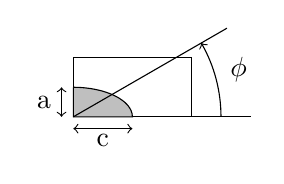
\begin{tikzpicture}
				\begin{scope}[scale=1.5]
				\draw (1,0.5) -- (2,0.5) -- (2,1) -- (1,1) -- (1,0.5);
				\draw[fill=gray!50] (1,0.75) arc (90:0:0.5 and 0.25) -- (1,0.5) -- (1,.75);
				\draw node at (1.25,0.3) {c};
				\draw node at (0.75,0.62) {a};
				\draw[<->] (1,0.4) -- (1.5,0.4);
				\draw[<->] (0.9,0.5) -- (0.9,0.75);
				\draw[thin] (1.75,0.5) -- (2.5,0.5);
				\draw[thin] (1,0.5) -- (2.3,1.25);
				\draw[->] (2.25,0.5) arc (0:30:1.25);
				\draw node at (2.4,0.9) {$\phi$};
				\end{scope}
				\end{tikzpicture}
			\end{figure}
			\begin{equation}
			K_I = \sigma \sqrt{\frac{\pi a}{Q}} \left[\sin^2 \phi + \frac{a^2}{c^2} \cos^2 \phi\right]^{1/4}(1.1)(1.1)
			\end{equation}
			Note: $1.1 \approx \sqrt{1.2}$, which is known as the front surface correction factor. A more accurate correction factor is given as
			\begin{equation*}
			1 + .12\left(1-\frac{a}{c}\right)
			\end{equation*}
		\end{column}
	\end{columns}
\end{frame}

\begin{frame}{semi-elliptical surface flaw in finite body}
	\begin{columns}[T]
		\begin{column}{0.40\columnwidth}
			\begin{figure}
				%\centering
				%\def\svgwidth{\columnwidth}
				%\input{3d_coord.pdf_tex}
				\tdplotsetmaincoords{75}{110}
				\begin{tikzpicture}[tdplot_main_coords,scale=1.5]
				\def\couleur{alerted text.fg}
				\def\altcouleur{example text.fg}
				\draw[fill=gray!50] (1,0.5,1) arc (270:90:0.25 and 0.5);
				\draw (1,0,0) -- (1,0,2) -- (1,2,2) -- (1,2,0) -- (1,0,0);
				\draw (1,2,0) -- (0,2,0) -- (0,2,2) -- (0,0,2) -- (1,0,2);
				\draw (1,2,2) -- (0,2,2);
				\draw [dashed] (0,0,2) -- (0,0,0) -- (0,2,0);
				\draw [dashed] (0,0,0) -- (1,0,0);
				\draw (1,0,1) -- (1,2,1) -- (0,2,1);
				\draw[dashed] (0,2,1) -- (0,0,1) -- (1,0,1);
				\end{tikzpicture}
			\end{figure}
		\end{column}
		\begin{column}{0.56\columnwidth}
			\begin{figure}
				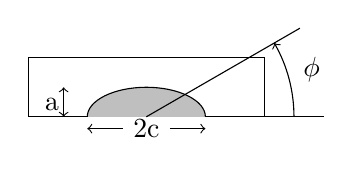
\begin{tikzpicture}
				\begin{scope}[scale=1.5]
				\draw (0,0.5) -- (2,0.5) -- (2,1) -- (0,1) -- (0,0.5);
				\draw[fill=gray!50] (.5,0.5) arc (180:0:0.5 and 0.25);
				\draw node at (1,0.4) {2c};
				\draw node at (0.2,0.6) {a};
				\draw[->] (1.2,0.4) -- (1.5,0.4);
				\draw[->] (0.8,0.4) -- (0.5,0.4);
				\draw[<->] (0.3,0.5) -- (0.3,0.75);
				\draw[thin] (1.75,0.5) -- (2.5,0.5);
				\draw[thin] (1,0.5) -- (2.3,1.25);
				\draw[->] (2.25,0.5) arc (0:30:1.25);
				\draw node at (2.4,0.9) {$\phi$};
				\end{scope}
				\end{tikzpicture}
			\end{figure}
			\begin{equation}
			K_I = \sigma \sqrt{\frac{\pi a}{Q}} \left[\sin^2 \phi + \frac{a^2}{c^2} \cos^2 \phi\right]^{1/4}(1.1) M_K
			\end{equation}
			Front surface correction same as for the infinite body.
			
			$M_K$ is the back surface correction, and can be looked up on a chart in your textbook.
		\end{column}
	\end{columns}
\end{frame}

\begin{frame}{finite thickness correction}
	\begin{figure}
		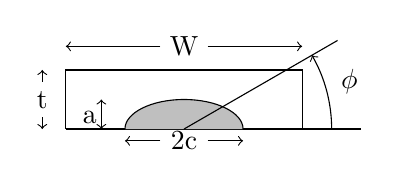
\begin{tikzpicture}
		\begin{scope}[scale=1.5]
		\draw (0,0.5) -- (2,0.5) -- (2,1) -- (0,1) -- (0,0.5);
		\draw[fill=gray!50] (.5,0.5) arc (180:0:0.5 and 0.25);
		\draw node at (1,0.4) {2c};
		\draw node at (0.2,0.6) {a};
		\draw[->] (1.2,0.4) -- (1.5,0.4);
		\draw[->] (0.8,0.4) -- (0.5,0.4);
		\draw[<->] (0.3,0.5) -- (0.3,0.75);
		\draw[thin] (1.75,0.5) -- (2.5,0.5);
		\draw[thin] (1,0.5) -- (2.3,1.25);
		\draw[->] (2.25,0.5) arc (0:30:1.25);
		\draw node at (2.4,0.9) {$\phi$};
		\draw node at (1,1.2) {W};
		\draw[->] (.8,1.2) -- (0,1.2);
		\draw[->] (1.2,1.2) -- (2,1.2);
		\draw node at (-0.2,.75) {t};
		\draw[->] (-.2,.9) -- (-0.2,1);
		\draw[->] (-.2,.6) -- (-0.2,.5);
		\end{scope}
		\end{tikzpicture}
	\end{figure}
	\begin{itemize}
		\item An alternative method for calculating the finite thickness and finite width correction factors uses the following formula
		\begin{equation}
		K_I = \sigma \sqrt{\pi c} \sqrt{\frac{a}{c Q^\prime}} \left[M_1 + \left(\sqrt{\frac{Q^\prime c}{a}}-M_1\right)\left(\frac{a}{t}\right)^P\right]\sqrt{\sec \left(\frac{\pi c}{W} \sqrt{\frac{a}{t}}\right)}
		\end{equation}
	\end{itemize}
\end{frame}

\begin{frame}{finite thickness correction}
	\begin{align*}
	M_1 &= 1.2 - 0.1 \frac{a}{c} & \text{for} \qquad 0.02 \le \frac{a}{c} \le 1\\
	&= \sqrt{\frac{c}{a}} \left(1 + 0.1 \frac{a}{c}\right) & \text{for} \qquad \frac{a}{c} > 1\\
	Q^\prime &= 1 + 1.47 \left(\frac{a}{c}\right)^{1.64} & \text{for} \qquad \frac{a}{c} \le 1\\
	&= 1 + 1.47 \left(\frac{c}{a}\right)^{1.64} & \text{for} \qquad \frac{a}{c} > 1\\
	P &= 2 + 8\left(\frac{a}{c}\right)^3
	\end{align*}
\end{frame}

\begin{frame}{cracks around a hole}
	\begin{figure}
		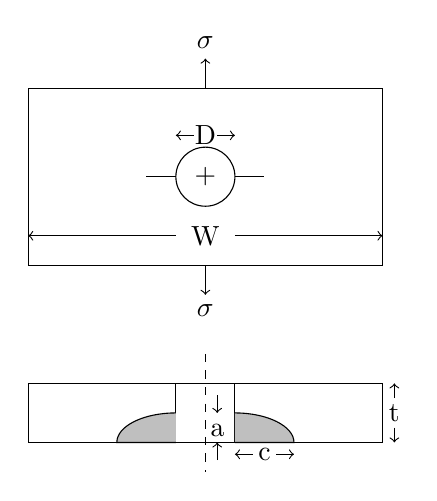
\begin{tikzpicture}
		\begin{scope}[scale=.75]
		\draw (0,-1.5) -- (0,1.5) -- (6,1.5) -- (6,-1.5) -- (0,-1.5);
		\draw[->] (3,1.5) -- (3,2) node[above] {$\sigma$};
		\draw[->] (3,-1.5) -- (3,-2) node[below] {$\sigma$};
		\draw (3,0) circle (0.5);
		\draw (3.5,0) -- (4,0);
		\draw (2.5,0) -- (2,0);
		\draw[->] (2.5,-1) -- (0,-1);
		\draw[->] (3.5,-1) -- (6,-1);
		\draw node at (3,-1) {W};
		\draw node at (3,0.7) {D};
		\draw node at (3,0) {+};
		\draw[->] (3.2,0.7) -- (3.5,0.7);
		\draw[->] (2.8,0.7) -- (2.5,0.7);
		\draw (0,-3.5) -- (6,-3.5) -- (6,-4.5) -- (0,-4.5) -- (0,-3.5);
		\draw[dashed] (3,-3) -- (3,-5);
		\draw (3.5,-3.5) -- (3.5,-4.5);
		\draw (2.5,-3.5) -- (2.5,-4.5);
		\draw node at (6.2,-4) {t};
		\draw node at (3.2,-4.3) {a};
		\draw node at (4,-4.7) {c};
		\draw[->] (6.2,-3.75) -- (6.2,-3.5);
		\draw[->] (6.2,-4.25) -- (6.2,-4.5);
		\draw[fill=gray!50] (3.5,-4) arc (90:0:1.0 and 0.5) -- (3.5,-4.5);
		\draw[fill=gray!50] (2.5,-4) arc (90:180:1.0 and 0.5) -- (2.5,-4.5);
		\draw[->] (4.2,-4.7) -- (4.5,-4.7);
		\draw[->] (3.8,-4.7) -- (3.5,-4.7);
		\draw[->] (3.2,-4.8) -- (3.2,-4.5);
		\draw[->] (3.2,-3.7) -- (3.2,-4.0);
		\end{scope}
		\end{tikzpicture}
	\end{figure}
\end{frame}

\begin{frame}{cracks around a hole}
	\begin{itemize}
		\item For corner cracks under uniform applied stress, we have
		\begin{align}
		\begin{split}
		K_I &= \sigma \sqrt{\pi c} \sqrt{\frac{a}{c Q^\prime}} \left[M_1 + \left(\sqrt{\frac{Q^\prime c}{a}}-M_1\right)\left(\frac{a}{t}\right)^P\right]\\
		&\sqrt{\sec \left(\frac{\pi}{2} \frac{D+bc}{W-2C+bc}\sqrt{\frac{a}{t}}\right)} f_b \sqrt{\sec \frac{\pi D}{2W}}
		\end{split}
		\end{align}
	\end{itemize}
\end{frame}

\begin{frame}{cracks around a hole}
	\begin{figure}
		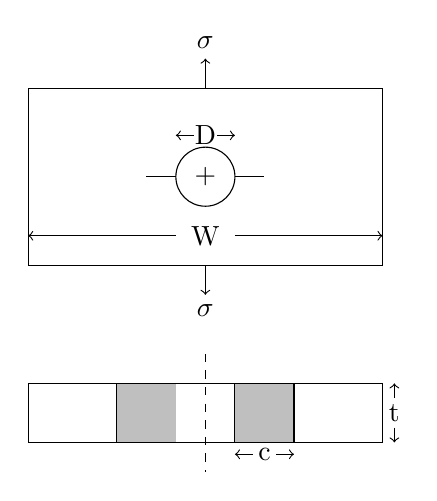
\begin{tikzpicture}
		\begin{scope}[scale=.75]
		\draw (0,-1.5) -- (0,1.5) -- (6,1.5) -- (6,-1.5) -- (0,-1.5);
		\draw[->] (3,1.5) -- (3,2) node[above] {$\sigma$};
		\draw[->] (3,-1.5) -- (3,-2) node[below] {$\sigma$};
		\draw (3,0) circle (0.5);
		\draw (3.5,0) -- (4,0);
		\draw (2.5,0) -- (2,0);
		\draw[->] (2.5,-1) -- (0,-1);
		\draw[->] (3.5,-1) -- (6,-1);
		\draw node at (3,-1) {W};
		\draw node at (3,0.7) {D};
		\draw node at (3,0) {+};
		\draw[->] (3.2,0.7) -- (3.5,0.7);
		\draw[->] (2.8,0.7) -- (2.5,0.7);
		\draw (0,-3.5) -- (6,-3.5) -- (6,-4.5) -- (0,-4.5) -- (0,-3.5);
		\draw[dashed] (3,-3) -- (3,-5);
		\draw (3.5,-3.5) -- (3.5,-4.5);
		\draw (2.5,-3.5) -- (2.5,-4.5);
		\draw node at (6.2,-4) {t};
		\draw node at (4,-4.7) {c};
		\draw[->] (6.2,-3.75) -- (6.2,-3.5);
		\draw[->] (6.2,-4.25) -- (6.2,-4.5);
		\draw[fill=gray!50] (3.5,-3.5) -- (4.5,-3.5) -- (4.5,-4.5) -- (3.5,-4.5);
		\draw[fill=gray!50] (2.5,-3.5) -- (1.5,-3.5) -- (1.5,-4.5) -- (2.5,-4.5);
		\draw[->] (4.2,-4.7) -- (4.5,-4.7);
		\draw[->] (3.8,-4.7) -- (3.5,-4.7);
		\end{scope}
		\end{tikzpicture}
	\end{figure}
\end{frame}

\begin{frame}{cracks around a hole}
	\begin{itemize}
		\item For through cracks under uniform applied stress, we have
		\begin{align}
		\begin{split}
		K_I &= \sigma \sqrt{\pi c}\sqrt{\sec \left(\frac{\pi}{2} \frac{D+bc}{W-2C+bc}\right)} f_b \sqrt{\sec \frac{\pi D}{2W}}
		\end{split}
		\end{align}
	\end{itemize}
\end{frame}

\begin{frame}{cracks around a hole}
	\begin{figure}
		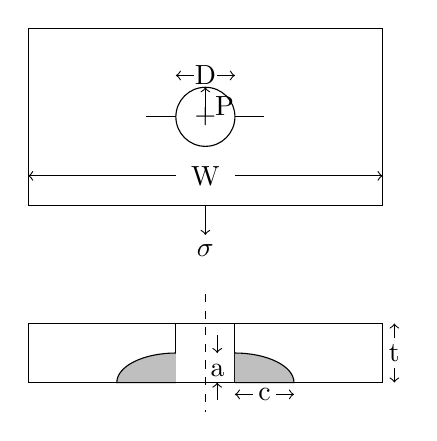
\begin{tikzpicture}
		\begin{scope}[scale=.75]
		\draw (0,-1.5) -- (0,1.5) -- (6,1.5) -- (6,-1.5) -- (0,-1.5);
		\draw[->] (3,0) -- (3,0.5) node[below right] {P};
		\draw[->] (3,-1.5) -- (3,-2) node[below] {$\sigma$};
		\draw (3,0) circle (0.5);
		\draw (3.5,0) -- (4,0);
		\draw (2.5,0) -- (2,0);
		\draw[->] (2.5,-1) -- (0,-1);
		\draw[->] (3.5,-1) -- (6,-1);
		\draw node at (3,-1) {W};
		\draw node at (3,0.7) {D};
		\draw node at (3,0) {+};
		\draw[->] (3.2,0.7) -- (3.5,0.7);
		\draw[->] (2.8,0.7) -- (2.5,0.7);
		\draw (0,-3.5) -- (6,-3.5) -- (6,-4.5) -- (0,-4.5) -- (0,-3.5);
		\draw[dashed] (3,-3) -- (3,-5);
		\draw (3.5,-3.5) -- (3.5,-4.5);
		\draw (2.5,-3.5) -- (2.5,-4.5);
		\draw node at (6.2,-4) {t};
		\draw node at (3.2,-4.3) {a};
		\draw node at (4,-4.7) {c};
		\draw[->] (6.2,-3.75) -- (6.2,-3.5);
		\draw[->] (6.2,-4.25) -- (6.2,-4.5);
		\draw[fill=gray!50] (3.5,-4) arc (90:0:1.0 and 0.5) -- (3.5,-4.5);
		\draw[fill=gray!50] (2.5,-4) arc (90:180:1.0 and 0.5) -- (2.5,-4.5);
		\draw[->] (4.2,-4.7) -- (4.5,-4.7);
		\draw[->] (3.8,-4.7) -- (3.5,-4.7);
		\draw[->] (3.2,-4.8) -- (3.2,-4.5);
		\draw[->] (3.2,-3.7) -- (3.2,-4.0);
		\end{scope}
		\end{tikzpicture}
	\end{figure}
\end{frame}

\begin{frame}{cracks around a hole}
	\begin{itemize}
		\item For corner cracks under fastener load, we have
		\begin{align}
		\begin{split}
		K_I &= \frac{P}{Wt} \sqrt{\pi c} \sqrt{\frac{a}{c Q^\prime}} \left[M_1 + \left(\sqrt{\frac{Q^\prime c}{a}}-M_1\right)\left(\frac{a}{t}\right)^P\right]\\
		&\sqrt{\sec \left(\frac{\pi}{2} \frac{D+bc}{W-2C+bc}\sqrt{\frac{a}{t}}\right)} f_b \sqrt{\sec \frac{\pi D}{2W}} G_b
		\end{split}
		\end{align}
	\end{itemize}
\end{frame}

\begin{frame}{cracks around a hole}
	\begin{figure}
		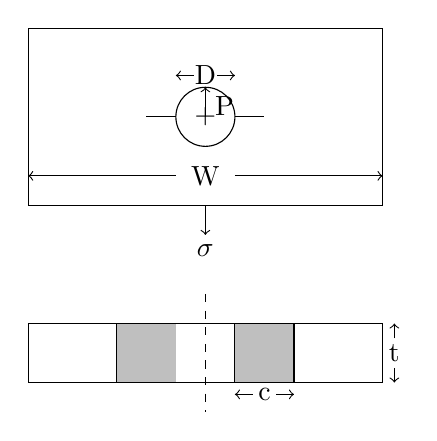
\begin{tikzpicture}
		\begin{scope}[scale=.75]
		\draw (0,-1.5) -- (0,1.5) -- (6,1.5) -- (6,-1.5) -- (0,-1.5);
		\draw[->] (3,0) -- (3,0.5) node[below right] {P};
		\draw[->] (3,-1.5) -- (3,-2) node[below] {$\sigma$};
		\draw (3,0) circle (0.5);
		\draw (3.5,0) -- (4,0);
		\draw (2.5,0) -- (2,0);
		\draw[->] (2.5,-1) -- (0,-1);
		\draw[->] (3.5,-1) -- (6,-1);
		\draw node at (3,-1) {W};
		\draw node at (3,0.7) {D};
		\draw node at (3,0) {+};
		\draw[->] (3.2,0.7) -- (3.5,0.7);
		\draw[->] (2.8,0.7) -- (2.5,0.7);
		\draw (0,-3.5) -- (6,-3.5) -- (6,-4.5) -- (0,-4.5) -- (0,-3.5);
		\draw[dashed] (3,-3) -- (3,-5);
		\draw (3.5,-3.5) -- (3.5,-4.5);
		\draw (2.5,-3.5) -- (2.5,-4.5);
		\draw node at (6.2,-4) {t};
		\draw node at (4,-4.7) {c};
		\draw[->] (6.2,-3.75) -- (6.2,-3.5);
		\draw[->] (6.2,-4.25) -- (6.2,-4.5);
		\draw[fill=gray!50] (3.5,-3.5) -- (4.5,-3.5) -- (4.5,-4.5) -- (3.5,-4.5);
		\draw[fill=gray!50] (2.5,-3.5) -- (1.5,-3.5) -- (1.5,-4.5) -- (2.5,-4.5);
		\draw[->] (4.2,-4.7) -- (4.5,-4.7);
		\draw[->] (3.8,-4.7) -- (3.5,-4.7);
		\end{scope}
		\end{tikzpicture}
	\end{figure}
\end{frame}

\begin{frame}{cracks around a hole}
	\begin{itemize}
		\item For through cracks under fastener load, we have
		\begin{align}
		\begin{split}
		K_I &= \frac{P}{Wt} \sqrt{\pi c}\sqrt{\sec \left(\frac{\pi}{2} \frac{D+bc}{W-2C+bc}\right)} f_b \sqrt{\sec \frac{\pi D}{2W}} G_b
		\end{split}
		\end{align}
	\end{itemize}
\end{frame}

\begin{frame}{cracks around a hole}
	\begin{align*}
	P &= 2+ 8\left(\frac{a}{c}\right)^3 & \qquad \lambda = \frac{1}{1+2C/D}\\
	M_1 &=1.2 - 0.1 \left(\frac{a}{c}\right) & \text{for} \qquad .02 \le \frac{a}{c} \le 1\\
	&= \sqrt{\frac{c}{a}} \left[1+ 0.1 \left(\frac{a}{c}\right)\right] & \text{for} \qquad \frac{a}{c} > 1\\
	f_b = f_1 &= .707 -.18\lambda + 6.55 \lambda^2 - 10.54 \lambda^3 + 6.85 \lambda^4 & \text{for} \qquad b=1\\
	f_b = f_2 &= 1 -.15\lambda + 3.46 \lambda^2 - 4.47 \lambda^3 + 3.52 \lambda^4 & \text{for} \qquad b=2\\
	G_1 &= \frac{1}{2} + \frac{W}{\pi (D+c)} \sqrt{\frac{D}{D+2c}} & \text{for} \qquad b=1\\
	G_2 &= \frac{1}{2} + \frac{W}{\pi (D+2c)} & \text{for} \qquad b=2\\
	\end{align*}
\end{frame}
\section{examples}
%Similar to HW 1-2
\begin{frame}{example 1}
	\begin{enumerate}
		\item 
		\begin{enumerate}
			\item Determine the value of $K_I$ for a center-cracked panel with $W/2a = 3$ and a uniformly applied remote stress, $\sigma$.
			\item Determine the value of $K_I$ for an edge-cracked panel with $W/a = 3$ and a uniformly applied remote stress, $\sigma$.
			\item Compare these two results. Note that in both cases the panel width to crack length ratio is the same.
		\end{enumerate}
	\end{enumerate}
\end{frame}

\begin{frame}{example 1}
	\begin{itemize}
		\item Based on the ratio of crack length to width, we choose (2) over (1)
		\begin{equation*}
		K_I = \sigma \sqrt{\pi a} \sqrt{\sec (\pi a/W)}
		\end{equation*}
		\item This gives $K_I = \sigma \sqrt{\pi a} \sqrt{\sec (\pi/6)}$
		\item If we normalize by the infinite width solution, we find $K_{I,f}/K_{I,i} \approx 1.075$
	\end{itemize}
\end{frame}

\begin{frame}{example 1}
	\begin{itemize}
		\item Once again, based on the ratio of crack length to width, we choose (4) over (3)
		\begin{equation*}
		K_I = \sigma \sqrt{\pi a}\left[1.12 - 0.231 \frac{a}{W} + 10.55 \left(\frac{a}{W}\right)^2 - 21.72 \left(\frac{a}{W}\right)^3 + 30.39 \left(\frac{a}{W}\right)^4\right]
		\end{equation*}
		\item This gives $K_I \approx 1.786 \sigma \sqrt{\pi a}$
		\item If we normalize by the infinite width solution, we find $K_{I,f}/K_{I,i} \approx 1.595$
	\end{itemize}
\end{frame}

\begin{frame}{example 1}
	\begin{itemize}
		\item Comparing the two cases, we see that the finite width effects are much more significant for the edge-crack specimen
		\item The edge-crack specimen is also overall more effected by a crack of that relative length.
		\item Why are they not the same?
	\end{itemize}
\end{frame}
%TODO FE simulation? (symmetry conditions)

%Similar to 1-4
\begin{frame}{example 2}
	\begin{columns}
		\begin{column}{0.45\textwidth}
			\begin{figure}[H]
				\centering
				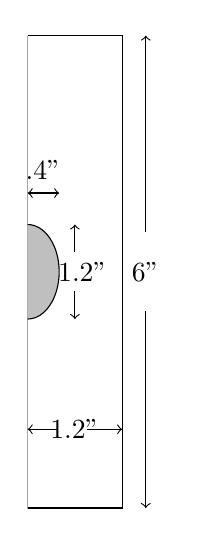
\begin{tikzpicture}
				\clip (0,3.1) rectangle (2.1,-3.1);
				\draw (0,3) -- (1.2,3) -- (1.2,-3) -- (0,-3) -- (0,3);
				\draw[fill=gray!50] (0,0) ellipse [x radius=0.4, y radius=0.6];
				\draw[->] (0.75,-2) node at (.6,-2) {1.2"} -- (1.2,-2); 
				\draw[->] (.39,-2) -- (0,-2);
				\draw[->] (0.6,-0.25) -- (0.6,-0.6) node at (0.7,0) {1.2"};
				\draw[->] (0.6,0.25) -- (0.6,0.6);
				\draw[<->] (0,1.0) -- (0.4,1.0);
				\draw node at (0.2, 1.3) {.4"};
				\draw[->] (1.5,0.5) -- (1.5,3);
				\draw[->] (1.5,-0.5) -- (1.5,-3);
				\draw node at (1.5,0) {6"};
				\end{tikzpicture}
				%\caption{Plate for Problem 4}
				\label{fig:problem4}
			\end{figure}
		\end{column}
		\begin{column}{0.45\textwidth}
			\begin{itemize}
				\item Find maximum value of $K_I$ for semi-elliptical surface flaw
				\item $\sigma = 20 \text{kpsi}$ (in opening direction)
			\end{itemize}
		\end{column}
	\end{columns}
\end{frame}

\begin{frame}{example 2}
	\begin{itemize}
		\item Here we will compare three different equations
		\item (8), which is for infinite width and thickness
		\begin{equation*}
		K_I = \sigma \sqrt{\frac{\pi a}{Q}} \left[\sin^2 \phi + \frac{a^2}{c^2} \cos^2 \phi\right]^{1/4}(1.1) \tag{8}
		\end{equation*}
		\item (10), which is for infinite width, but finite thickness
		\begin{equation*}
		K_I = \sigma \sqrt{\frac{\pi a}{Q}} \left[\sin^2 \phi + \frac{a^2}{c^2} \cos^2 \phi\right]^{1/4}(1.1) M_K \tag{10}
		\end{equation*}
		\item And (11), which accounts for finite width and thickness
		\begin{equation*}
		K_I = \sigma \sqrt{\pi c} \sqrt{\frac{a}{c Q^\prime}} \left[M_1 + \left(\sqrt{\frac{Q^\prime c}{a}}-M_1\right)\left(\frac{a}{t}\right)^P\right]\sqrt{\sec \left(\frac{\pi c}{W} \sqrt{\frac{a}{t}}\right)} \tag{11}
		\end{equation*}
	\end{itemize}
\end{frame}
\end{document}
